\documentclass[journal,12pt,twocolumn]{IEEEtran}
\usepackage{graphicx}
\graphicspath{{./figs/}}{}
\usepackage{amsmath,amssymb,amsfonts,amsthm}
\newcommand{\myvec}[1]{\ensuremath{\begin{pmatrix}#1\end{pmatrix}}}
\providecommand{\norm}[1]{\lVert#1\rVert}
\usepackage{listings}
\usepackage{watermark}
\usepackage{titlesec}
\usepackage{caption}
\usepackage{gensymb}
\newcommand{\mydet}[1]{\ensuremath{\begin{vmatrix}#1\end{vmatrix}}}
\let\vec\mathbf
\lstset{
frame=single, 
breaklines=true,
columns=fullflexible
}
\thiswatermark{\centering \put(0,-105.0){
\includegraphics[scale=0.15]{logo.png}} }
\title{\mytitle}
\title{
Assignment - 12.11.1.1
}
\author{Surajit Sarkar}
\begin{document}
\maketitle
\tableofcontents
\bigskip
\section{\textbf{Problem}}
The perpendicular distance from the origin is 5 units and the angle made by the perpendicular with the positive x-axis is $30^{\circ}$.Find the equation of the line ?
\section{\textbf{Solution}}
\begin{align}
\vec{m}&=\myvec{1\\\tan30^{\circ}}\\
\vec{n}&=\myvec{1\\\frac{1}{\sqrt{3}}}\\
\vec{P}&=\frac{10}{\sqrt{3}}
\end{align}
Equation
\begin{align}
    \vec{n}^{\top}\myvec{\vec{x}-\vec{P}}&=0\\
    \myvec{1&\frac{1}{\sqrt{3}}}\vec{x}&=\frac{10}{\sqrt{3}}\\
    \myvec{\sqrt{3}&1}\vec{x}&=10
\end{align}
\section{\textbf{Code Link}}
\begin{lstlisting}
https://github.com/sssurajit/fwc/blob/main/lines/11.10.2.8/codes/code.py
\end{lstlisting}
Execute the code by using the command\\
\textbf{python3 code.py}\\
\section{\textbf{Figure}}
\begin{figure}[!h]
\centering
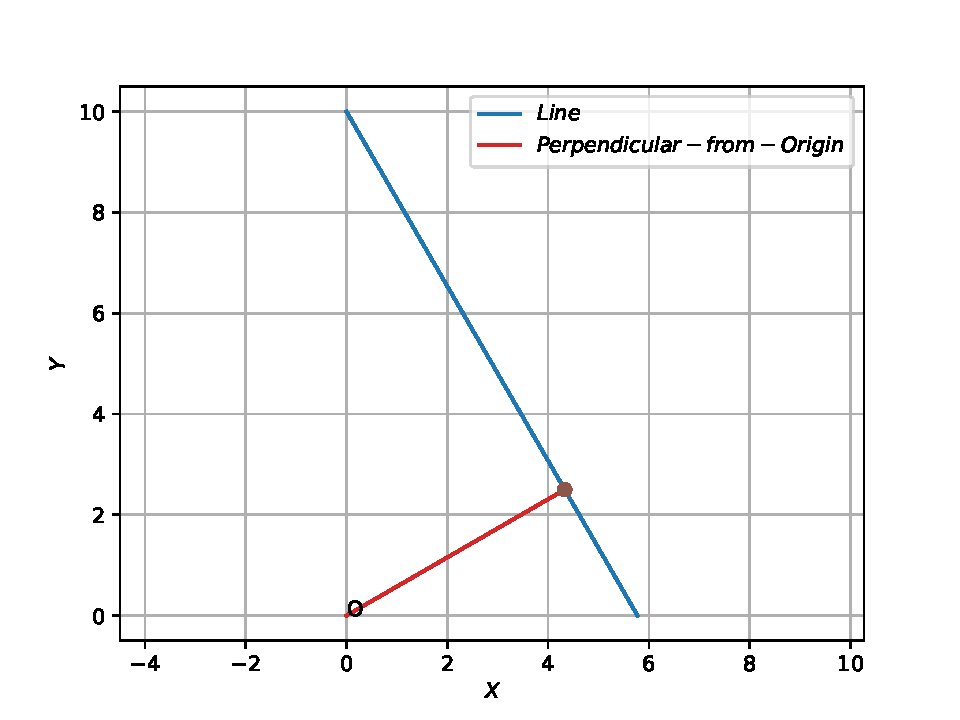
\includegraphics[width=\columnwidth]{fig.pdf}
\caption{}
\label{fig:vec}
\end{figure}
\end{document}

